\documentclass[10pt,twocolumn,letterpaper]{article}

\usepackage{cvpr}
\usepackage{times}
\usepackage{epsfig}
\usepackage{graphicx}
\usepackage{amsmath}
\usepackage{amssymb}
\usepackage[sorting=none]{biblatex}
\addbibresource{egbib.bib}
\graphicspath{{img/}}


% Include other packages here, before hyperref.

% If you comment hyperref and then uncomment it, you should delete
% egpaper.aux before re-running latex.  (Or just hit 'q' on the first latex
% run, let it finish, and you should be clear).
\usepackage[breaklinks=true,bookmarks=false]{hyperref}

\cvprfinalcopy % *** Uncomment this line for the final submission

\def\cvprPaperID{****} % *** Enter the CVPR Paper ID here
\def\httilde{\mbox{\tt\raisebox{-.5ex}{\symbol{126}}}}

% Pages are numbered in submission mode, and unnumbered in camera-ready
%\ifcvprfinal\pagestyle{empty}\fi
\setcounter{page}{1}
\begin{document}

%%%%%%%%% TITLE
\title{Machine learning project: Speech recognition challenge}

\author{Massimiliano Conte\\
{\tt\small massimiliano.conte.2@studenti.unipd.it}
% For a paper whose authors are all at the same institution,
% omit the following lines up until the closing ``}''.
% Additional authors and addresses can be added with ``\and'',
% just like the second author.
% To save space, use either the email address or home page, not both
\and
Pierpaolo D'Odorico\\
{\tt\small pierpaolo.dodorico@studenti.unipd.it}
}

\maketitle
%\thispagestyle{empty}

%%%%%%%%% ABSTRACT
%\begin{abstract}
%   The ABSTRACT is to be in fully-justified italicized text, at the top
%   of the left-hand column, below the author and affiliation
%   information. Use the word ``Abstract'' as the title, in 12-point
%   Times, boldface type, centered relative to the column, initially
%   capitalized. The abstract is to be in 10-point, single-spaced type.
%   Leave two blank lines after the Abstract, then begin the main text.
%   Abstract should be no longer than 300 words.
%\end{abstract}

%%%%%%%%% BODY TEXT
\section{Introduction}

The faced problem is the speech recognition challenge, where the goal is to build a system that can automatically recognize spoken words. In particular, the spoken words are given as input in form of audio recordings of one second length, while the output of the system is the text of the recognized words. All the recordings are waveform of one of the following 8 words:
\begin{itemize}
	\itemsep-0.3em 
	\item Down;
	\item Go;
	\item Left;
	\item Off;
	\item On;
	\item Right;
	\item Stop;
	\item Up.
\end{itemize}
This task is a key component in many artificial intelligence services, such as virtual assistants, and more generally speech recognition is part of the natural language processing domain.\\
Our work begin after the features extraction provided us by the professors, in form of log mel-spectrogram, that is a bi-dimensional representation of the recordings, involving frequency and time. After that, the images of the spectrograms are first resized and than reshaped in 1024-dimensional vectors.\\
We have faced the problem by applying several machine learning methods, from the easier ones to the more complicated ones, and choosing the best performing method based on accuracy. This led us to a system capable of classifying spoken words with an accuracy of more that 95\%. 

\section{Dataset}

The used dataset is a reduced version of TensorFlow Speech Commands Dataset v0.0.1 \cite{tensorflow2015-whitepaper}. The data provided us is alredy divided in training and validation set. The training set is composed of 1600 samples, 200 for each of the 8 classes, and the validation set is composed of 109 samples.
Every recording has a sampling frequency of 16 kHz. The hop length used for constructing the log Mel-spectrogram is 512, while it is not specified the window size. The feature extraction mimics the humany auditory system, providing a representation of the audio taking into account the fact that humans perceve both the frequencies and the amplitude of the sound logarithmically. The whole preocess of extracting the features for each recording can be summarized in:
\begin{itemize}
	%\itemsep0em 
	\item \textbf{Create the windows}, by sampling the recording and making hops of size 512;
	\item \textbf{Compute the discrete Fuorier transform} for each window, using the fast Fourier transform algorithm;
	\item \textbf{Convert to the Mel scale}: changing the representation from of the frequencies from Hz to the Mel scale (the scale of pitches judged by listeners to be equal in distance one from another, a kind of human perceving frequency scale);
	\item \textbf{Create the features}, by computing the log Mel-spectrogram (that is an image), resizing and reshaping it to a 1024 dimensional vector.
\end{itemize}
The dataset provided us alredy contains the extracted features and the correct class of the samples. The dataset doesn't have unbalanced classes problem.

\section{Method}
The methods used in this project are machine learning tecniques that are well suited for multiclass classification tasks. We tried the performance of various methods under different configurations, starting from the basic models and ending with the more complicated ones. Many models we tried are based on binary classification, the way we used such models are using the one-vs-all strategy, i. e. training one binary classifier per class and than predict the instances by loocking at the classifier that maximizes the confidence score.
\subsection{List of used methods}
Every method can be tuned by changing some hyperparameters. In the following table we reported the tecniques, which of those hyperparameters we taked into account for selecting the best configuration, and how that method handle multiclass classification.\\
\begin{table}[h!]
	\begin{center}
		\resizebox{\columnwidth}{!}{
		\begin{tabular}{|c|c|c|}
			\hline
			Method & Hyperparameters & handling \\
			\hline\hline
			
			
			
			Linear Classification & C : Regularization & One-vs-all \\
			
			\hline
			Logistic Regression & C : Regularization & One-vs-all \\
			
			\hline
			K-Neighbors Classifier  & K : number of neighbors & Majority vote of  \\
			&& the K-neighbors \\
			
			\hline
			Classification tree & Max depth; & Naturally handle multiclass \\
			&Min samples leaf;&\\
			&Min impurity decrease&\\
			
			\hline
			Random forest & Number of trees & Naturally handle multiclass \\
			
			\hline
			Support Vector Machine & C : Regularization; & One-vs-all \\
			&Type of kernel&\\
			
			\hline
			Neural network &  & Softmax activation \\
			&&on the output layer\\ 
			
			\hline
		\end{tabular}}
	\end{center}
	\caption{List of used methods.}
	\label{mytable}
\end{table}
\\
All the methods are implementes using \textit{Python} \cite{van1995python} and \textit{Sklearn} \cite{scikit-learn}, exept for the neural networks where we used \textit{Keras} \cite{chollet2015keras}. The host for the challenge is \textit{Kaggle} \cite{kaggle}.

\subsection{Metodology}
For every listed method we first set a grid of hyperparameters configurations, then trained one model for each configuration and then choosed the best performing one. For fairness reasons, we didn't use the validation set for choosing the best configuration, keeping the validation set unseen by the models until the decision of the overall best performing method.\\ In particular, we divided the training set in two parts, a sort of training and validation sets for the hyperparameter search. The models were trained on the "little" training set and the best configuration was choosen on the "little" validation set, by looking at the highest accuracy.
Then the model is trained again on the entire training set, using the found configuration, in order to take advantage of all the data.\\
Once that we found the best configuration for each model, we used the unseen validation set for choosing the overall best method.\\ Usually, this kind of split is referred as training, validation and test set, but here the set used as test set was alredy named validation set.
\section{Experiments}
In this section we describe the hyperparameters we choosed and show, where it is possible with graphs, what's the best configuration that we found. After that, we compare the methods accuracy on the validation set.
\subsection{Linear classification}
The Hyperparameter used in this method is \textit{alpha}, a regularization tuner. The larger \textit{alpha}, the stronger the regularization. It refers to the \textit{l2}, which is the standard regularizer based on the euclidian norm of the parameters vector.
\begin{figure}[h!]
	\centering
	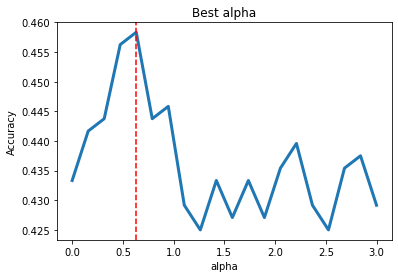
\includegraphics[width=6cm]{LC.png}
	\caption{Accuracy as the intensity of the regularization varies.}
	\label{LC.png}
\end{figure}
\medskip

\subsection{Logistic regression}
The Hyperparameter used in this method is \textit{C}, which has a similar role as the \textit{alpha} decribed before, tuning the intensity of the regularization. The larger the \textit{C}, the weaker the regularization. Can be seen as $\frac{1}{alpha}$.
\begin{figure}[h!]
	\centering
	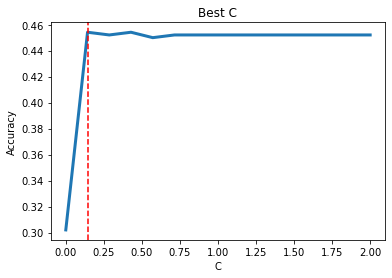
\includegraphics[width=6cm]{LR.png}
	\caption{Accuracy as the intensity of the regularization varies.}
	\label{LR.png}
\end{figure}
\medskip

\subsection{KNN}
The Hyperparameter used in this method is \textit{K}, the number of neirest neighbors examined for the majority vote.
\begin{figure}[h!]
	\centering
	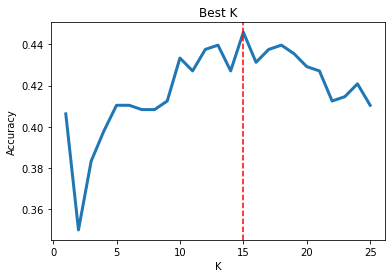
\includegraphics[width=6cm]{KNN.png}
	\caption{Accuracy as the number of the considered neighbors varies.}
	\label{KNN.png}
\end{figure}
\medskip

\subsection{Decision tree}
The criterion used for measuring the impurity on the leafs is the gini impuruty:\\ $G(leaf) = \sum_{i = 1}^{8}n(i, leaf) (1 - n(i, leaf)) $ where $n(i, leaf)$ is the number of samples in the $leaf$ that belong to the $i$-th class. \\The Hyperparameters used in this method are:
\begin{itemize}
	%\itemsep-0.3em 
	\item \textit{Max depth};
	\item \textit{Min samples leaf}, the minimum number of samples required for each leaf;
	\item \textit{Min impurity decrease}, the minimum decrease of impurity required for each split.
\end{itemize}
The best configuration found is:

\begin{itemize}
	%\itemsep-0.3em 
	\item \textit{Max depth} = 9;
	\item \textit{Min samples leaf} = 2;
	\item \textit{Min impurity decrease} = 0.00316.
\end{itemize}

\subsubsection{Random forest}
This method is the aggragation of \textit{n trees}, where each was trained on a different set, obtained via bootstrap replications of the training set. \textit{n trees} was set to be 1000. Each tree uses the previous found best hyperparameter configuration.

\subsection{Support vector machine}
The Hyperparameters used in this method are:
\begin{itemize}
	%\itemsep-0.3em 
	\item \textit{C}, the same regularization parameter as before;
	\item \textit{Kernel}, the type of kernel used by the method, choosed between polynomial or gaussian.
\end{itemize}
\begin{figure}[h!]
	\centering
	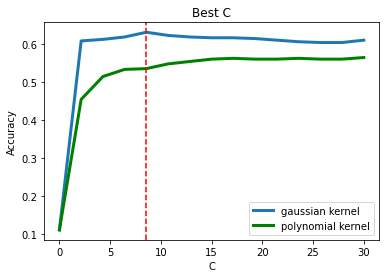
\includegraphics[width=6cm]{SVM.png}
	\caption{Accuracy for polynomial and gaussian kernels as the intensity of the regularization varies.}
	\label{SVM.png}
\end{figure}
\subsection{Neural network}








%{\small
%\bibliographystyle{ieee_fullname}
%\bibliography{egbib}
%}

\newpage

\printbibliography

\end{document}
